\section{Results}
\label{sec:physical_regimes}

Even in this simplest possible case, the physics of the reduced system is startlingly rich. The exact solution of the previous section therefore invites a detailed numerical analysis. With the exact form of the mean-force state, we can precisely characterise the behaviour of the system in different regimes of temperature and bath coupling. 

First, to expose the coupling dependence cleanly, we reintroduce an explicit dimensionless strength $g$ by writing the bath kernel as
\begin{equation}
    K(u)=g^2 K_0(u).
\end{equation}
All response kernels inherit the same quadratic scaling, such that
\begin{equation}
    \Delta_z \to g^2 \Delta_{z},
    \qquad
    \Sigma_\pm \to g^2 \Sigma_{\pm},
    \qquad
    \chi \to g^2 \chi,
\end{equation}
The entire non-perturbative recombination of bare Hamiltonian and influence is therefore controlled by the single dimensionless dressing parameter $\chi$ through
\begin{equation}
    \gamma(\chi)=\frac{\tanh\chi}{\chi}.
    \label{eq:gamma_chi_validation}
\end{equation}

This apparently innocuous expression encodes the entire non-perturbative recombination of bare Hamiltonian and influence, and functions as an \emph{order} parameter for the crossover between weak and ultrastrong coupling regimes. The reduced equilibrium state transitions between these regimes as $\chi$ passes through unity,
\begin{equation}
    \chi(\beta,g,\theta)\sim 1
    \qquad \Longleftrightarrow \qquad
    g^2 \sim \chi_0(\beta,\theta)^{-1}.
    \label{eq:chi_crossover_condition_v5}
\end{equation}


This crossover condition $\chi(\beta,g,\theta)=1$ therefore
defines a coupling-dependent temperature scale
\begin{equation}
  g_\star(\beta) = \chi_0(\beta,\theta)^{-1/2},
  \label{eq:gstar_def_v6}
\end{equation}
and an equivalent crossover temperature $\beta_\star(g)$.  No approximation has
been made; $g_\star$ is an exact property of the solution.

The function $\gamma(\chi)$ is elementary but worth dwelling on.  It is
monotone decreasing from $\gamma(0)=1$ to $\gamma(\infty)=0$, with curvature
that changes sign near $\chi\approx 1.2$.  In the two limiting regimes:
\begin{align}
  \chi \ll 1:\quad & \gamma \simeq 1 - \tfrac{\chi^2}{3},
  \label{eq:gamma_weak}\\
  \chi \gg 1:\quad & \gamma \simeq \chi^{-1} = (g^2\chi_0)^{-1}.
  \label{eq:gamma_strong}
\end{align}

The exact formulas of Sec.~\ref{subsec:qubit_exact_geometry} contain three
distinct physical phenomena that are absent from the bare-Gibbs or
weak-coupling pictures.  We examine each in turn.

\subsection{The running coupling and temperature-driven crossover}
\label{subsec:running_coupling}

From Eq.~\eqref{eq:chi_factored}, the crossover parameter factorises as
$\chi = g^2\chi_0(\beta)$, where the bath susceptibility $\chi_0(\beta)$ is
the $g$-independent part.  For an Ohmic bath $J(\omega) = \alpha\omega
e^{-\omega/\omega_c}$, $\chi_0(\beta)$ is a monotone increasing function of
$\beta$: the bath accumulates more imaginary-time dressing as the temperature
decreases.  This means that for any fixed coupling $g$, the dimensionless
expansion parameter $\chi$ \emph{grows} as the system cools, crossing through
the non-perturbative scale $\chi\sim 1$ at the crossover temperature
\begin{equation}
    \beta_\star(g) \;\text{ defined by }\; \chi_0(\beta_\star) = g^{-2}.
\end{equation}
The coupling $g$ thus plays the role of a renormalization-group bare coupling,
and $\chi(\beta,g)$ is the corresponding running coupling at scale $\beta$: the
system flows from a weak-coupling fixed point at high temperature to a
strong-coupling regime upon cooling.

Figure~\ref{fig:running_coupling} illustrates this for three representative
couplings.  Panel~(a) shows $\chi(\beta)$ rising through the crossover line
$\chi=1$ at $\beta_\star(g)$ (filled circles).  Panels~(b) and~(c) show the
corresponding evolution of the Bloch angle $\varphi$ and Bloch radius $r$: both
quantities track their bare values for $\beta < \beta_\star(g)$ (high temperature,
weak coupling) and acquire significant strong-coupling corrections for
$\beta > \beta_\star(g)$ (low temperature, strong coupling).  The onset is smooth
--- it is controlled by the regular function $\gamma(\chi) = \tanh\chi/\chi$ ---
but the corrections accelerate steeply once $\chi \gg 1$.

\begin{figure}[t]
    \centering
    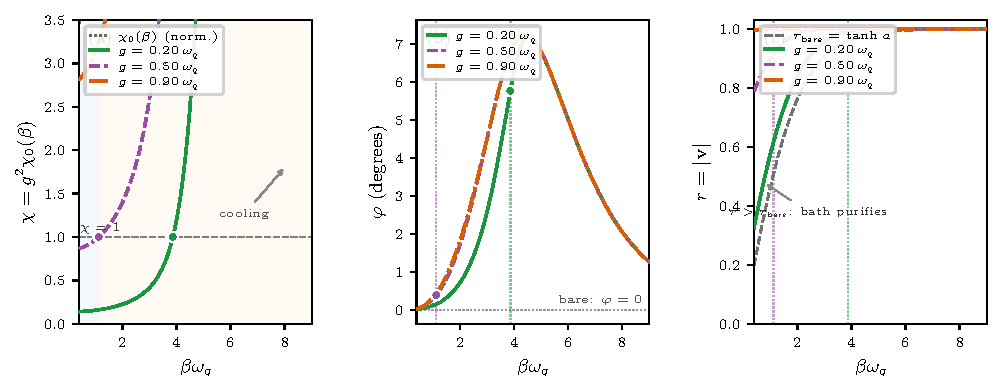
\includegraphics[width=\columnwidth]{../figures/hmf_running_coupling.pdf}
    \caption{Temperature-driven crossover for three coupling strengths
    ($g = 0.20, 0.50, 0.90\,\omega_q$; Ohmic bath, $\theta=\pi/6$).
    \textbf{(a)} Running coupling $\chi(\beta) = g^2\chi_0(\beta)$ versus
    $\beta\omega_q$.  The dotted baseline shows the bath susceptibility
    $\chi_0(\beta)$ (same shape for all $g$, scaled by $g^2$). Filled circles
    mark the crossover temperature $\beta_\star(g)$ where $\chi=1$.
    \textbf{(b)} Bloch angle $\varphi = \arctan(m_x, -m_z)$ (deviation from the
    bare thermal axis $-\hat{\mathbf{n}}_s$).  The angle accumulates below
    $\beta_\star$ and saturates at the strong-coupling attractor direction.
    \textbf{(c)} Bloch radius $r = |\mathbf{r}|$, with the bare thermal purity
    $r_{\rm bare} = \tanh(\beta\omega_q/2)$ (black dashed) as a reference.
    For this Ohmic bath (bandwidth $2\omega_q$) the mean-force radius exceeds
    $r_{\rm bare}$ at all temperatures: the bath always purifies.  The excess
    is largest at high temperature ($\beta$ small, left of each $\beta_\star$
    marker) where the bare state is nearly mixed, and smallest at low
    temperature where the bare state is already near-pure.}
    \label{fig:running_coupling}
\end{figure}


\begin{figure}[ht]
    \centering
    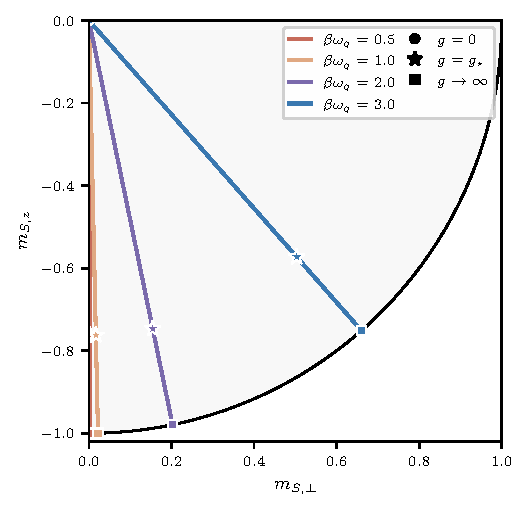
\includegraphics[width=0.98\columnwidth]{../figures/hmf_bloch_disk_portrait.pdf}
    \caption{Influence of the bath coupling on the qubit equilibrium state.
    \textbf{(a)} Trajectory of the exact mean-force Bloch vector in the coupling 
    plane for $\theta = \pi/4$ (Ohmic bath, $\alpha=1$, 
    $\omega_c = 5\,\omega_q$). To resolve the non-perturbative divergence 
    at weak coupling, we plot the longitudinal polarization $m_z = \langle\sigma_z\rangle$ 
    against the square-root transverse polarization $\sqrt{m_x} = \sqrt{\langle\sigma_x\rangle}$. 
    Curves correspond to temperatures $\beta\omega_q \in \{0.5, 1.0, 2.0, 3.0\}$. 
    Markers indicate the bare thermal state (circle), the crossover 
    $g = g_\star$ (star), and the strong-coupling attractor (square). 
    The solid black line denotes the physical purity boundary $r=1$ in the 
    transformed coordinate system.
    \textbf{(b)} Bloch radius $r$ as a function of the normalized coupling 
    $g/g_\star(\beta)$, resolving the crossover from weak ($g < g_\star$) 
    to strong ($g > g_\star$) regimes (shaded). Dotted horizontals 
    show the bare thermal purity $r_{\rm bare} = \tanh(\beta\omega_q/2)$. 
    Coupling to the bath always increases the qubit purity ($r > r_{\rm bare}$), 
    with the strongest effect at high temperatures where the bare state is 
    near the maximally-mixed center of the disk.}
    \label{fig:bloch_disk_portrait}
\end{figure}

\subsection{Purity of the mean-force state}
\label{subsec:purity}

The purity of the qubit mean-force state is $\mathcal{P} = \tfrac{1}{2}(1 +
r^2)$ with $r^2 = |\mathbf{r}|^2$.  We can establish an exact, universal
result:
\begin{quote}
\textbf{Bath always purifies.} \textit{For any positive spectral density
$J(\omega)\geq 0$ and any coupling $g>0$ and temperature $\beta>0$,}
\begin{equation}
    r^2(g,\beta) \;>\; r_{\rm bare}^2 \;=\; \tanh^2\!\left(\frac{\beta\omega_q}{2}\right),
    \label{eq:purity_bound}
\end{equation}
\textit{with equality only at $g=0$.}
\end{quote}

\paragraph{Proof sketch.}
The key ingredient is the sign of the longitudinal channel amplitude $\Delta_{z,0}$.
Writing the imaginary-time bath kernel $K(u)\geq 0$, the channel amplitude is
\begin{equation}
    \Delta_{z,0} = \frac{s^2}{\pi}\int_0^\beta ({\beta}-u)\,K(u)\,\sinh(\omega_q u)\,du.
\end{equation}
All three factors in the integrand are non-negative on $[0,\beta]$
(since $\beta - u \geq 0$, $\sinh(\omega_q u) \geq 0$), so $\Delta_{z,0} > 0$
and therefore $n_z = -\Delta_{z,0}/\chi_0 < 0$.

With $n_z < 0$, direct computation of $r^2 - \tanh^2 a$ from the exact
Bloch vector formula gives the numerator
\begin{equation}
    \mathcal{N} \;=\; \sinh^2\!\chi\bigl(n_z^2\sinh^2\!a + \cosh^2\!a\bigr)
    - n_z\,\sinh(2a)\,\tfrac{\sinh(2\chi)}{2} > 0,
\end{equation}
since both terms are positive when $n_z < 0$ and $a,\chi > 0$.  The
denominator is manifestly positive, so $r^2 > \tanh^2 a$. $\square$

\paragraph{Limits.}
At $a\to 0$ (infinite temperature) the bare state is maximally mixed but the
coupling gives
\begin{equation}
    r\big|_{a=0} = \tanh\chi > 0,
    \label{eq:purity_highT}
\end{equation}
and at $\chi\to\infty$ (very strong coupling) one finds $r\to 1$ (pure state)
regardless of temperature.  Thus the mean-force state interpolates from the
mixed bare state to a pure state as coupling increases, for any bath spectral
function and any temperature.

The result is independent of the bandwidth or spectral shape of $J(\omega)$;
widening the bandwidth increases $\chi_0(\beta)$ (driving the system to the
strong-coupling regime at weaker $g$) but never reverses the purity inequality.
Purity inversion would require $n_z > 0$, i.e.\ a bath kernel with negative
imaginary-time correlations, which is impossible for any physical (positive)
spectral density.

\paragraph{Purity landscape.}
Figure~\ref{fig:purity_landscape} displays the purity excess
$\Delta r^2 = r^2 - \tanh^2 a > 0$ throughout the $(g,\beta)$ plane for the
Ohmic bath parameters used throughout.  Panel~(a) shows the absolute purity
$r^2$; the white dashed contour is the crossover locus $\chi=1$.  Panel~(b)
shows $\Delta r^2$: the enhancement peaks at large $g$ and high temperature
(upper-right), where the bath lifts the near-maximally-mixed bare state far
above its uncoupled value.  At low temperature (bottom) the bare state is
already near-pure and the excess vanishes.

\begin{figure}[t]
    \centering
    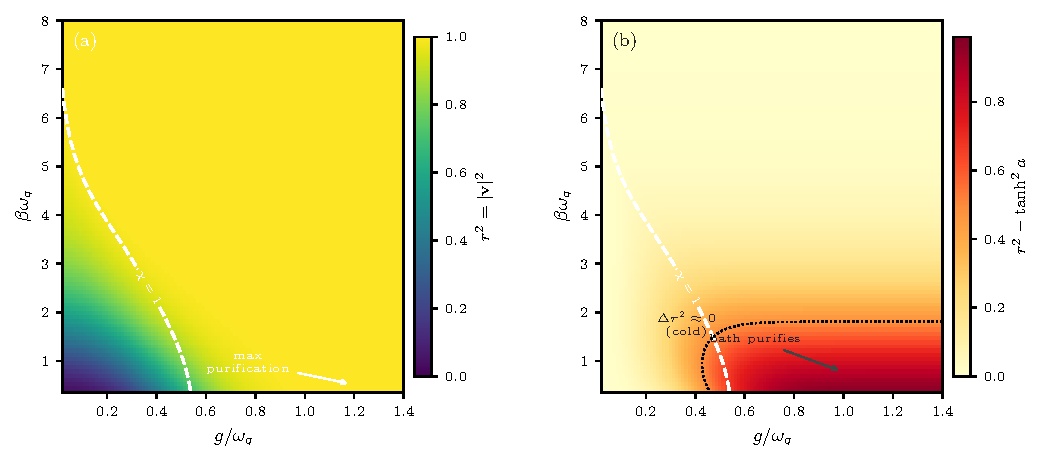
\includegraphics[width=\columnwidth]{../figures/hmf_purity_landscape.pdf}
    \caption{Purity of the qubit mean-force state in the $(g,\beta)$ plane
    ($\theta=\pi/6$, Ohmic bath).
    \textbf{(a)} Absolute purity $r^2 = |\mathbf{r}|^2$.  The white dashed
    contour marks $\chi=1$ (crossover locus).
    \textbf{(b)} Purity excess $\Delta r^2 = r^2 - \tanh^2 a > 0$ (sequential
    colour scale).  By the exact result Eq.~\eqref{eq:purity_bound}, coupling always increases
    purity for any harmonic bath; the maximum enhancement is at large $g$ and
    high temperature, where the bath selects a preferred pure state from the
    near-maximally-mixed bare thermal ensemble.}
    \label{fig:purity_landscape}
\end{figure}

\subsection{Geometry of the state trajectory}
\label{subsec:trajectory}

The preceding analysis is unified by the Bloch disk portrait in
Fig.~\ref{fig:bloch_disk_portrait}.  Several features of that figure deserve
emphasis.

\paragraph{Temperature-dependent attractors.}
The squares in panel~(a) (large-$g$ attractors for each temperature) lie at
\emph{different} points on or near the unit circle boundary.  This is because
the direction $\hat{\mathbf h}_{\mathrm{eff}}$ depends on temperature through
$b_{\rm nr}(\beta)$ and $b_{\rm r}(\beta)$: the bath-channel weights are
frequency-resolved spectral integrals that change with $\beta$.  By contrast,
the Cresser--Anders ultrastrong limit predicts a \emph{single} attractor
direction aligned with $\hat{\mathbf f}$ (shown as the gray arrow) independent
of temperature.  The temperature-dependence of the exact attractor is the
\emph{temperature memory} of the mean-force state: even at arbitrarily strong
coupling, the state encodes information about the temperature.

\paragraph{Purity along the trajectory.}
Panel~(b) shows $r(g/g_\star)$ for each temperature.  The dotted horizontal
lines are $r_{\rm bare} = \tanh a$.  By Eq.~\eqref{eq:purity_bound}, every
trajectory lies strictly above its own $r_{\rm bare}$ line for all $g > 0$.
The effect is most visible at high temperature ($\beta\omega_q=0.5$, red),
where the bare state is near the maximally-mixed center and the bath-selected
pure-state attractor offers a large purity gain.  At low temperature
($\beta\omega_q=6$, dark blue) the bare state is already near-pure and the
excess is correspondingly small, though still nonzero.  All trajectories
converge to $r\to 1$ (pure state) as $g\to\infty$, consistent with the
universal strong-coupling limit identified above.

\paragraph{Non-commutativity of limits.}
The limits $g\to\infty$ and $T\to 0$ do not commute.  Taking $g\to\infty$ at
fixed $T > 0$ locks the state to the bath-dressed attractor direction with
finite-temperature purity.  Taking $T\to 0$ at fixed $g$ instead sends
$a\to\infty$, and the state approaches the ground state $-\hat{\mathbf{n}}_s$
regardless of $g$.  These two operations access qualitatively different corners
of the state space.


\subsection{Relation to weak- and ultrastrong-coupling mean-force results}
\label{subsec:qubit_relation_to_limits}

It is useful to make explicit how the exact qubit geometry derived above relates
to the weak- and ultrastrong-coupling mean-force Gibbs (MFG) results in the
literature, in particular the qubit limit discussed by Cresser and Anders.  Their
central ultrastrong statement is a \emph{basis-selection} result: as the coupling
scale $\lambda\to\infty$, the MFG state becomes diagonal in the eigenbasis of
the coupling operator $X$, rather than in the bare Hamiltonian basis
$H_Q$~\cite{cresserWeakUltrastrongCoupling2021a}.  For a qubit with coupling axis $\hat{\mathbf
f}$ and bare Hamiltonian axis $\hat{\mathbf{n}}_s$, this yields a limiting state whose
Bloch vector points along $\hat{\mathbf f}$ (with a temperature-dependent
magnitude set by the projected bare splitting).

Our exact Gaussian qubit solution is not in contradiction with that result, but
it resolves a different structure. The qubit geometry obtained here proceeds in
two distinct steps:
\begin{equation}
(\hat{\mathbf{n}}_s,\hat{\mathbf f};\text{bath}) \;\longmapsto\; \mathbf h_{\mathrm{eff}}
\;\longmapsto\; \mathbf r .
\end{equation}
The first map constructs a \emph{bath-dressed influence direction} through the
symmetrised exponent, Eq.~\eqref{eq:heff_def}, which is explicitly anisotropic
in the pair of directions $\{\hat{\mathbf f}_\perp,\hat{\mathbf{n}}_s\}$, with separate
weights carried by the non-resonant and resonant bath channels.  The second map
then combines this dressed influence with the bare Gibbs factor $\Pi$ to
produce the final Bloch vector $\mathbf r$.  The bath does not merely rescale
$\hat{\mathbf f}$; it remaps the coupling geometry relative to the system axis before
thermal recombination.

Rewriting $\mathbf h_{\mathrm{eff}}$ in the coupling-adapted frame with
$c\equiv \cos\theta$, $s\equiv \sin\theta$:
\begin{equation}
\mathbf h_{\mathrm{eff}}
=
s^2 c\,(\Sigma_z - \Sigma_\perp)\,\hat{\mathbf f}
+
s\,(\Sigma_\perp c + \Sigma_z s^2)\,\hat{\mathbf n}^{(f)}_\perp ,
\label{eq:heff_coupling_frame}
\end{equation}
where $\hat{\mathbf n}^{(f)}_\perp \equiv (\hat{\mathbf{n}}_s-c\hat{\mathbf f})/s$.
The coupling-axis ultrastrong geometry of Cresser--Anders is recovered only when $\mathbf h_{\mathrm{eff}}$ aligns with $\hat{\mathbf f}$. From Eq.~\eqref{eq:heff_coupling_frame}, this requires the resonant and non-resonant bath channels to satisfy a specific ratio that compensates for the coupling's geometric anisotropy:
\begin{equation}
\frac{\Sigma_z}{\Sigma_\perp} = -\frac{c}{s^2}
\label{eq:ultrastrong_alignment_condition}
\end{equation}
(or equivalently $\Sigma_\perp c + \Sigma_z s^2 = 0$).
which is a special condition on the bath parameters. Absent
Eq.~\eqref{eq:ultrastrong_alignment_condition}, the exact Gaussian qubit state
may still enter the strong-coupling crossover (large $\chi$), but approaches a
bath-dressed attractor direction rather than the bare coupling axis itself (see
the squares in Fig.~\ref{fig:bloch_disk_portrait}a).

A useful summary is therefore:
\begin{quote}
The Cresser--Anders ultrastrong theorem identifies the asymptotic \emph{basis}
selected in the singular coupling limit, while the present exact qubit geometry
resolves the \emph{route} to strong coupling in terms of a bath-anisotropic
dressed influence vector built from resonant and non-resonant channels.
\end{quote}
